% ============================================================
%  Chapter 4 — Implementation
% ============================================================
\chapter{Implementation}
\label{ch:implementation}

This chapter covers the full set of loss terms used during training
(\secref{sec:losses}), the training datasets and how we prepare them
(\secref{sec:data}), and the optimisation schedule that controls which losses
and datasets are active at each stage (\secref{sec:schedule}).
Every value in this chapter is taken directly from the training configuration
used to produce the final model.


\section{Loss Terms}
\label{sec:losses}

Our model is trained with three families of losses: \emph{supervised anchors}
that tie the predictions to ground-truth labels on synthetic data, \emph{CARI
losses} that enforce illuminant invariance on real multi-illuminant pairs, and
\emph{physics and regularisation terms} that keep the decomposition consistent.
The total loss is a weighted sum; \tabref{tab:losses} lists every active term
with its weight.

\begin{table}[t!]
  \caption[Training loss terms and weights.]{%
    Loss terms used in training, with the weights of the final
    configuration.
    Supervised anchors require ground-truth labels and are gated to the
    synthetic datasets that provide them; CARI terms require multi-illuminant
    pairs and fire only on MID batches during the CARI stage; physics terms
    apply only where their required targets and masks exist.
    A gradient-decorrelation loss (forcing albedo and shading edges apart) was
    evaluated and \emph{rejected}: it assumes albedo and shading edges never
    coincide, which is false in real scenes, and it erased genuinely shared
    edges.
  }
  \label{tab:losses}
  \centering
  \small
  \begin{tabular}{@{}llcl@{}}
    \toprule
    Loss term & Symbol & Weight & Applies to \\
    \midrule
    Albedo $\ell_1$              & $\mathcal{L}_{\text{a}}$        & 1.0  & Hypersim, IV, MID (pseudo-GT) \\
    Albedo DSSIM                 & $\mathcal{L}_{\text{dssim}}$    & 0.2  & same as $\mathcal{L}_{\text{a}}$ \\
    Albedo multi-scale gradient  & $\mathcal{L}_{\text{msg-a}}$    & 0.5  & same as $\mathcal{L}_{\text{a}}$ \\
    Albedo chroma direction      & $\mathcal{L}_{\text{chroma}}$   & 0.2  & same as $\mathcal{L}_{\text{a}}$ \\
    Shading SSI ($\pi$-domain)   & $\mathcal{L}_{\text{s}}$        & 1.0  & Hypersim (GT shading) \\
    Shading multi-scale gradient & $\mathcal{L}_{\text{msg-s}}$    & 0.5  & Hypersim \\
    Diffuse reconstruction       & $\mathcal{L}_{\text{recon}}$    & 1.0  & Hypersim \\
    Reconstruction gradient      & $\mathcal{L}_{\text{msg-r}}$    & 0.25 & Hypersim \\
    Residual closure + sparsity  & $\mathcal{L}_{\text{res}}$      & 0.5 / 0.02 & Hypersim, MID \\
    Material consistency (DINO)  & $\mathcal{L}_{\text{mat}}$      & 0.05 & all datasets \\
    Cross-render invariance      & $\mathcal{L}_{\text{inv}}$      & 0.5  & MID raw pairs \\
    Shading explanation          & $\mathcal{L}_{\text{expl}}$     & 0.25 & MID raw pairs \\
    Shading sign prior           & $\mathcal{L}_{\text{sign}}$     & 0.05 & all datasets \\
    \bottomrule
  \end{tabular}
\end{table}


\subsection{Supervised Anchor Losses}

\paragraph{Albedo ($\mathcal{L}_{\text{a}}$, $\mathcal{L}_{\text{dssim}}$,
$\mathcal{L}_{\text{msg-a}}$, $\mathcal{L}_{\text{chroma}}$)}
The core albedo supervision is a masked $\ell_1$ loss against the ground-truth
albedo $\mathbf{A}^*$:
\begin{equation}
  \mathcal{L}_{\text{a}} =
  \frac{1}{|\Omega_m|}\sum_{p \in \Omega_m}
  \bigl\| \mathbf{A}(p) - \mathbf{A}^*(p) \bigr\|_1
  \label{eq:l_albedo}
\end{equation}
where $\Omega_m$ excludes invalid pixels (missing labels, clipped regions).
This is the dominant \emph{absolute-colour anchor} of the whole system: CARI
constrains albedo to be equal \emph{across} illuminants but says nothing about
what the correct colour \emph{is}; without a strong absolute anchor, the
invariance constraint alone could be satisfied by grey.
Three companions sharpen this anchor.
A structural dissimilarity term $\mathcal{L}_{\text{dssim}}$ (DSSIM, weight 0.2)
penalises local structure differences.
A multi-scale gradient term $\mathcal{L}_{\text{msg-a}}$ (weight 0.5) matches
predicted albedo gradients to ground-truth gradients across four dyadic scales,
placing each edge where the ground truth says it belongs.
Finally, a \emph{chroma-direction} term (weight 0.2),
\begin{equation}
  \mathcal{L}_{\text{chroma}} =
  \frac{1}{|\Omega_m|}\sum_{p \in \Omega_m}
  \Bigl\| \tfrac{\mathbf{A}(p)}{\|\mathbf{A}(p)\|} -
          \tfrac{\mathbf{A}^*(p)}{\|\mathbf{A}^*(p)\|} \Bigr\|_1 ,
  \label{eq:l_chroma}
\end{equation}
penalises hue and saturation error independently of brightness.
This term exists because desaturation is the cheap escape for a pixel-wise loss:
predicting a slightly grey version of every colour lowers $\ell_1$ risk, and
$\mathcal{L}_{\text{chroma}}$ makes that escape expensive.

\paragraph{Shading SSI ($\mathcal{L}_{\text{s}}$, $\mathcal{L}_{\text{msg-s}}$)}
Shading is only defined up to an arbitrary global scale: a dimmer light with
a brighter material explains the same image. The renderer's absolute
light intensity varies freely between scenes, so a naive regression to
ground-truth shading would spend most of its gradient fighting a quantity
that is not identifiable.
The standard remedy, introduced for the analogous scale ambiguity in
monocular depth estimation \mycite{ranftl20midas} and adopted for shading by
\mycitetext{careaga23ordinal}, is a \emph{scale-and-shift-invariant} (SSI)
loss: before the error is computed, the prediction is aligned to the ground
truth with the per-image scalar scale $\hat{s}$ and shift $\hat{t}$ that
minimise the squared error, a two-parameter least-squares problem with a
closed-form solution, so the alignment adds no optimisation difficulty.
The aligned prediction is then penalised with a masked mean-squared error in
the bounded $\boldsymbol{\pi}$ domain:
\begin{equation}
  \mathcal{L}_{\text{s}} =
  \frac{1}{|\Omega_d|}\sum_{p \in \Omega_d}
  \bigl( \hat{s}\,\boldsymbol{\pi}(p) + \hat{t} - \boldsymbol{\pi}^*(p) \bigr)^2 ,
  \qquad
  (\hat{s}, \hat{t}) = \arg\min_{s,t} \sum_{p \in \Omega_d}
  \bigl( s\,\boldsymbol{\pi}(p) + t - \boldsymbol{\pi}^*(p) \bigr)^2
  \label{eq:l_shade}
\end{equation}
$\Omega_d$ is the \emph{diffuse mask}: shading ground truth exists only on
Hypersim, so this loss is gated to Hypersim batches.
This supervises the relative shading pattern (shadows, gradients) without being
confused by per-scene brightness.
A multi-scale gradient companion (weight 0.5) sharpens shading boundaries.
The SSI alignment is enabled after a 3{,}000-iteration warm-up, during which the
un-aligned loss stabilises the output range first.

\paragraph{Diffuse reconstruction ($\mathcal{L}_{\text{recon}}$,
$\mathcal{L}_{\text{msg-r}}$)}
Because the residual is analytic ($\mathbf{R} = (\mathbf{I} - \mathbf{A}\odot\mathbf{S}_d)_+$),
a naive reconstruction loss $\|\mathbf{A}\odot\mathbf{S}_d + \mathbf{R} - \mathbf{I}\|$
would be identically zero wherever the diffuse product undershoots the image, which is a
tautology that provides no gradient.
We therefore supervise the \emph{diffuse product} directly:
\begin{equation}
  \mathcal{L}_{\text{recon}} =
  \frac{1}{|\Omega_d|}\sum_{p \in \Omega_d}
  \bigl\| \mathbf{A}(p) \odot \mathbf{S}_d(p) -
          \mathbf{A}^*(p) \odot \mathbf{S}^*_d(p) \bigr\|_1
  \label{eq:l_recon}
\end{equation}
The term is enabled only for Hypersim, where the target is the measured
ground-truth diffuse product. It is a \emph{two-sided} coupling: both predicted
factors must jointly explain $\mathbf{A}^*\odot\mathbf{S}^*_d$. InteriorVerse and
MID do not activate this loss in the implemented configuration; those batches
are supervised by their available albedo, material, residual, sign, and CARI
terms instead. This masking is important: defining an input-derived target for
datasets without measured shading would change the trained objective.

\paragraph{Residual closure ($\mathcal{L}_{\text{res}}$)}
The analytic residual creates an escape hatch: the model could dump hard-to-
explain image content (for example a saturated red surface) into $\mathbf{R}$
instead of the albedo.
We close it with a supervised residual block (weight 0.5): on Hypersim the
residual target is the true non-diffuse component of the rendering, and on MID
the target is $\mathbf{R}^* = 0$ away from specular pixels (physically true for
the bounced-flash captures), so the loss there penalises \emph{any} residual
energy.
A small sparsity term (weight 0.02) additionally pushes $\mathbf{R} \to 0$
inside the valid mask, so the diffuse product rather than the residual must explain
the image.

\subsection{CARI Losses}

The two CARI losses $\mathcal{L}_{\text{inv}}$ (weight 0.5) and
$\mathcal{L}_{\text{expl}}$ (weight 0.25) are defined in \secref{sec:cari}.
They are computed by running the network a second time on the paired frame
$\mathbf{I}_2$ within the same training step (a Siamese second forward with
shared weights) and are masked by the intersection of the loss mask, the
material-invariance mask, and the per-pair HDR validity mask.
They fire on batches that contain MID raw pairs, i.e.\ from the CARI stage
onwards (\secref{sec:schedule}).

\subsection{Physics and Regularisation Losses}

\paragraph{Shading sign prior ($\mathcal{L}_{\text{sign}}$)}
The analytic residual is clamped non-negative, so any pixel where the diffuse
product \emph{overshoots} the image is un-modelled negative energy, which is something
the decomposition cannot represent.
The sign prior penalises exactly that overshoot:
\begin{equation}
  \mathcal{L}_{\text{sign}} =
  \frac{1}{|\Omega_m|}\sum_{p \in \Omega_m}
  \bigl\| \max\bigl(\mathbf{A}(p) \odot \mathbf{S}_d(p) - \mathbf{I}(p),\, 0\bigr) \bigr\|_1
  \label{eq:l_sign}
\end{equation}
The intuition is ``anything that brightens the image beyond the light must come
from the material, not the shading'': the term pushes brightening texture out of
the shading and into the albedo, complementing CARI (which pushes illuminant
colour out of the albedo and into the shading).

\paragraph{Material consistency ($\mathcal{L}_{\text{mat}}$)}
The frozen DINOv2 tokens provide a label-free material signal: two patches with
very similar tokens are very likely the same material.
The material-consistency term (weight 0.05) penalises albedo chroma differences
between patch pairs whose DINOv2 similarity exceeds a threshold, gently
flattening the albedo \emph{within} a material while leaving material boundaries
untouched.
Since the tokens are computed anyway for the encoder, this supervision is
essentially free.


\section{Training Data}
\label{sec:data}

Four datasets participate in training, each with a distinct role. In this
chapter, \emph{dataset} means a collection from which training samples are drawn.
It does not mean an evaluation procedure. Chapter~5 uses held-out data together
with a fixed protocol and metric; that combination is a \emph{benchmark}. MID
appears in both roles, but its training and test scenes are disjoint.
Three are existing public corpora and carry the two-stage schedule of
\secref{sec:schedule}: Hypersim and InteriorVerse supply supervised albedo, and
MID supplies the real cross-render pairs that CARI trains on.
The fourth, 3D-Front-IID (\secref{sec:front3d}), is rendered for this thesis to
supply the one combination none of the others offers: a large, deliberately
coloured illuminant change \emph{and} a ground-truth albedo for the same camera.
It enters at the refinement stage, where \secref{sec:lever_sweep} studies its
contribution in an exploratory configuration comparison.

\subsection{Hypersim}

Hypersim \mycite{roberts21hypersim} is a large photorealistic synthetic dataset
of 461 indoor scenes generated with a physically-based renderer, providing
ground-truth albedo (diffuse reflectance) and diffuse illumination for every
image.
It is the primary source of supervised signal: albedo, shading, reconstruction,
and residual targets all come from Hypersim labels.
The full release is large (multiple terabytes of EXR renders); under a local
storage budget of 500\,GB we download and train on approximately one quarter of
the scenes, sampled across the scene split so that the material and layout
diversity is preserved.
This subset is sufficient because Hypersim's role is to anchor absolute albedo
colour and supply shading ground truth, not to cover every scene; the
cross-illuminant signal that the thesis depends on comes from the real MID pairs
(\secref{sec:mid_dataset}), not from Hypersim.
We use the standard scene split within the subset and hold out a validation set
for monitoring and checkpoint selection.

\subsection{InteriorVerse}

InteriorVerse \mycite{zhu22interiorverse} is a rendered indoor dataset with
ground-truth material, geometry, and spatially varying lighting annotations.
It enters training as \emph{albedo-supervision diversity}: more scenes, layouts,
and materials for the absolute-colour anchor.
Its shading is defined only implicitly ($\mathbf{S}^*_d = \mathbf{I}/\mathbf{A}^*$),
so it is excluded from both shading-GT and diffuse-reconstruction losses in the
implemented configuration. InteriorVerse contributes albedo supervision and
material diversity, rather than a separately measured diffuse-image target.

\subsection{MID: Real Multi-Illuminant Pairs}

MID \mycite{midintrinsics} provides the cross-render training signal: over
1{,}000 real indoor scenes, each captured 25 times with a flash bounced in a
different direction, pixel-aligned, with the 30 test scenes held out
(\secref{sec:mid_dataset}).
Each MID training sample contributes two things:

\emph{(i) A supervised primary frame.}
The MID Intrinsics extension of \mycitetext{careaga23ordinal} supplies a dense
pseudo-ground-truth albedo per scene, derived from the white-balanced
multi-illumination stack; it is not part of the original MID release.
The white-balanced primary frame is supervised against this pseudo-GT with the
standard albedo losses, which anchors absolute colour on real photographs.

\emph{(ii) A raw cross-render pair.}
A second frame of the same scene, under a different bounce direction, is loaded
\emph{raw}, without white balance, together with a per-pair HDR validity mask
that drops pixels clipped or near-black in either frame.
The CARI losses operate on this pair.
As established in \secref{sec:cari}, disabling white balance here is essential
(the \texttt{mid\_raw\_color\_pair} flag): the measured 15--25\% illuminant
chromaticity variation across bounce directions \emph{is} the training signal,
and white balance would erase it.
An earlier configuration approximated this signal with synthetic chromatic
augmentation (random global tints on the pair frame); it measurably hurt
constancy on ARAP, because the synthetic tint distribution does not match real
illuminants, and it was replaced by the raw pairs.
\figref{fig:mid_preprocessing} summarises this preprocessing split: the
white-balanced primary frame provides the supervised colour anchor, while the raw
paired frames preserve the illuminant change used by CARI.

\begin{figure}[t!]
  \centering
  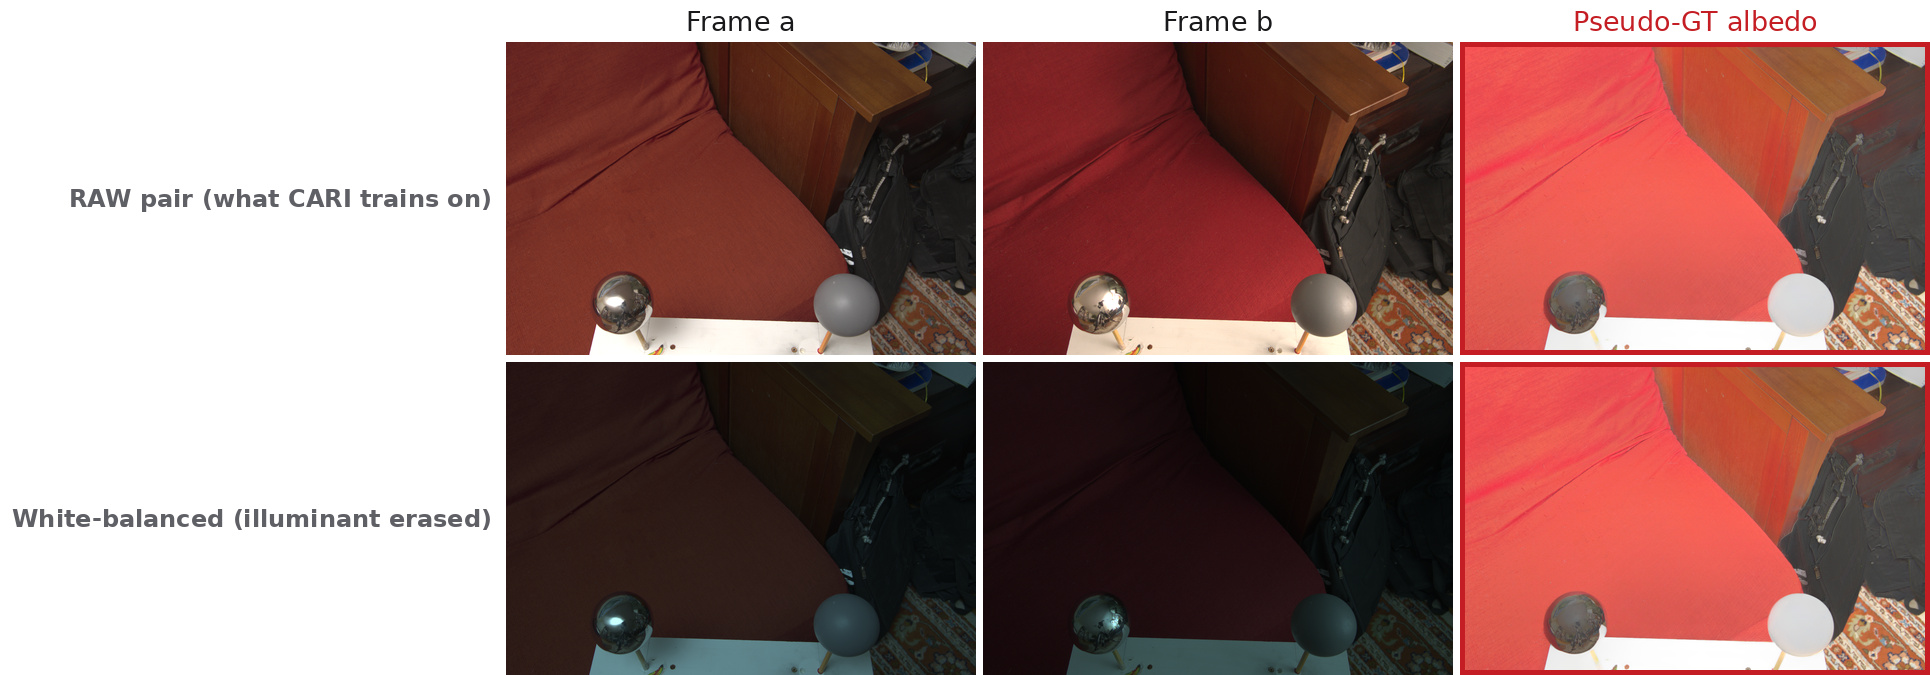
\includegraphics[width=0.92\textwidth]{images/hires/mid_preprocessing.jpg}
  \caption[MID training preprocessing paths.]{%
    MID preprocessing used during training; this is a data-loading diagram, not
    an evaluation protocol.
    The supervised path uses a white-balanced primary frame and the dataset
    pseudo-ground-truth albedo to anchor absolute material colour on real
    photographs.
    The CARI path keeps two aligned frames raw, without white balance, and masks
    pixels that are clipped or too dark in either exposure before applying the
    cross-render losses.
    This split keeps the albedo target stable while preserving the illuminant
    chromaticity change that CARI needs as supervision.
  }
  \label{fig:mid_preprocessing}
\end{figure}

\subsection{3D-Front-IID: A Rendered Cross-Illuminant Corpus}
\label{sec:front3d}

\paragraph{Motivation: the gap MID cannot close}
MID is the only \emph{real} source of cross-render pairs available to CARI, and
the thesis depends on it, but it constrains the method along two axes at once.
First, MID varies the illuminant by bouncing a single flash in a different
\emph{direction}: what changes most between two frames is the geometry and
intensity of the light, and only incidentally its colour, whose chromaticity
moves by roughly 15--25\% across bounce directions (\secref{sec:mid_dataset}).
The literal claim of this thesis is about \emph{coloured} illumination, and the
one dataset that supervises it does so only weakly and indirectly.
Second, MID has no measured dense albedo: its pseudo-ground-truth is itself
derived from the white-balanced capture stack.
On a MID pair the invariance loss therefore acts without an independent
absolute anchor on the same pixels, so nothing in the pair itself prevents the
two predictions from agreeing on a \emph{wrong} albedo; the anchor has to
arrive from a different dataset, on a different image.
The synthetic corpora have the opposite problem: Hypersim and InteriorVerse
supply exact albedo, but each image is a single illumination, so they carry no
cross-render signal at all.

Among the public datasets available to this project, none offered both
properties together. We therefore rendered one.

\paragraph{How it is built}
3D-Front-IID is rendered from 3D-FRONT \mycite{fu213dfront}, a corpus of
professionally designed indoor layouts furnished with 3D-FUTURE assets, using
Blender's Cycles path tracer at $512\times512$ and 64 samples per pixel
(\texttt{scripts/render\_3dfront\_dataset.py}).
Four design decisions define it.

\begin{itemize}
  \item \textbf{Interior camera sampling.}
        The layouts ship with exterior ``dollhouse'' camera poses, which are
        unusable as photographs.
        Cameras are instead sampled \emph{inside} each room and accepted by ray
        casting a grid through the frustum: a view is kept only if it is not
        embedded in geometry, is not staring at a blank wall or the ceiling,
        and actually frames furniture rather than empty floor.
  \item \textbf{Randomised coloured illuminants: the thesis axis.}
        Each accepted view is rendered under $K \in \{2,3\}$ lighting variants
        from the identical camera. Every variant re-randomises a key light
        (a blackbody between 2500\,K and 9000\,K, or a saturated hue) together
        with a near-neutral fill, and a \emph{minimum rg-chromaticity gap} is
        enforced between the key lights of a view.
        The illuminant colour is thus a controlled, guaranteed-present variable
        rather than a by-product: every pair the loader can draw is a genuine
        colour change, by construction.
  \item \textbf{Exact albedo, pixel-aligned.}
        After the lit passes, every material is converted to an emission shader
        and all lights are removed, so the renderer returns each surface's base
        colour directly. The result is a true ground-truth albedo registered
        pixel-for-pixel with every lit variant of that view.
  \item \textbf{Automatic quality control.}
        Each rendered view is validated for exposure clipping, black frames,
        valid-pixel coverage and framing, and failures are quarantined rather
        than trained on; 103 of 2{,}599 rendered views were dropped this way.
\end{itemize}

The resulting corpus contains 960 rooms and 2{,}496 accepted views, yielding
\textbf{5{,}056 cross-illuminant pairs}. The illuminant separation is wide and
guaranteed: the median rg-chromaticity distance between the two illuminants of
a pair is $0.23$, and no pair falls below the enforced floor of $0.055$.
\figref{fig:front3d} shows samples together with the measured illuminant gamut
and pair-separation distribution.

\paragraph{What the corpus is designed to test}
A 3D-Front-IID sample is the only one in the mix where the cross-render pair and
an exact albedo target coexist \emph{on the same pixels}: the loader returns two
lit observations, the ground-truth albedo, and a per-pair validity mask.
Two things follow.
The invariance loss and the supervised albedo anchor act on the same image, so
the degenerate solution available on an unanchored pair, in which two predictions
drift together onto a consistent but incorrect albedo, is directly
penalised rather than left to a different dataset to correct.
And because the varied quantity is illuminant \emph{colour} by construction,
CARI is supervised on the axis the thesis actually claims, instead of inferring
it from a direction change that only partly implies it.
Its shading, like InteriorVerse's, is defined only implicitly as
$\mathbf{S}^*_d = \mathbf{I}/\mathbf{A}^*$, so 3D-Front-IID is excluded from the
shading-ground-truth-gated losses; it contributes the albedo anchor and the CARI
pair, not a shading target.
\secref{sec:lever_sweep} measures what this contributes by adding the corpus to
the training mix as one arm of an exploratory comparison. The configurations
differ in more than one lever, so this study motivates a conclusion about the
combined training recipe rather than a single-cause estimate of the corpus.

\begin{figure}[t!]
  \centering
  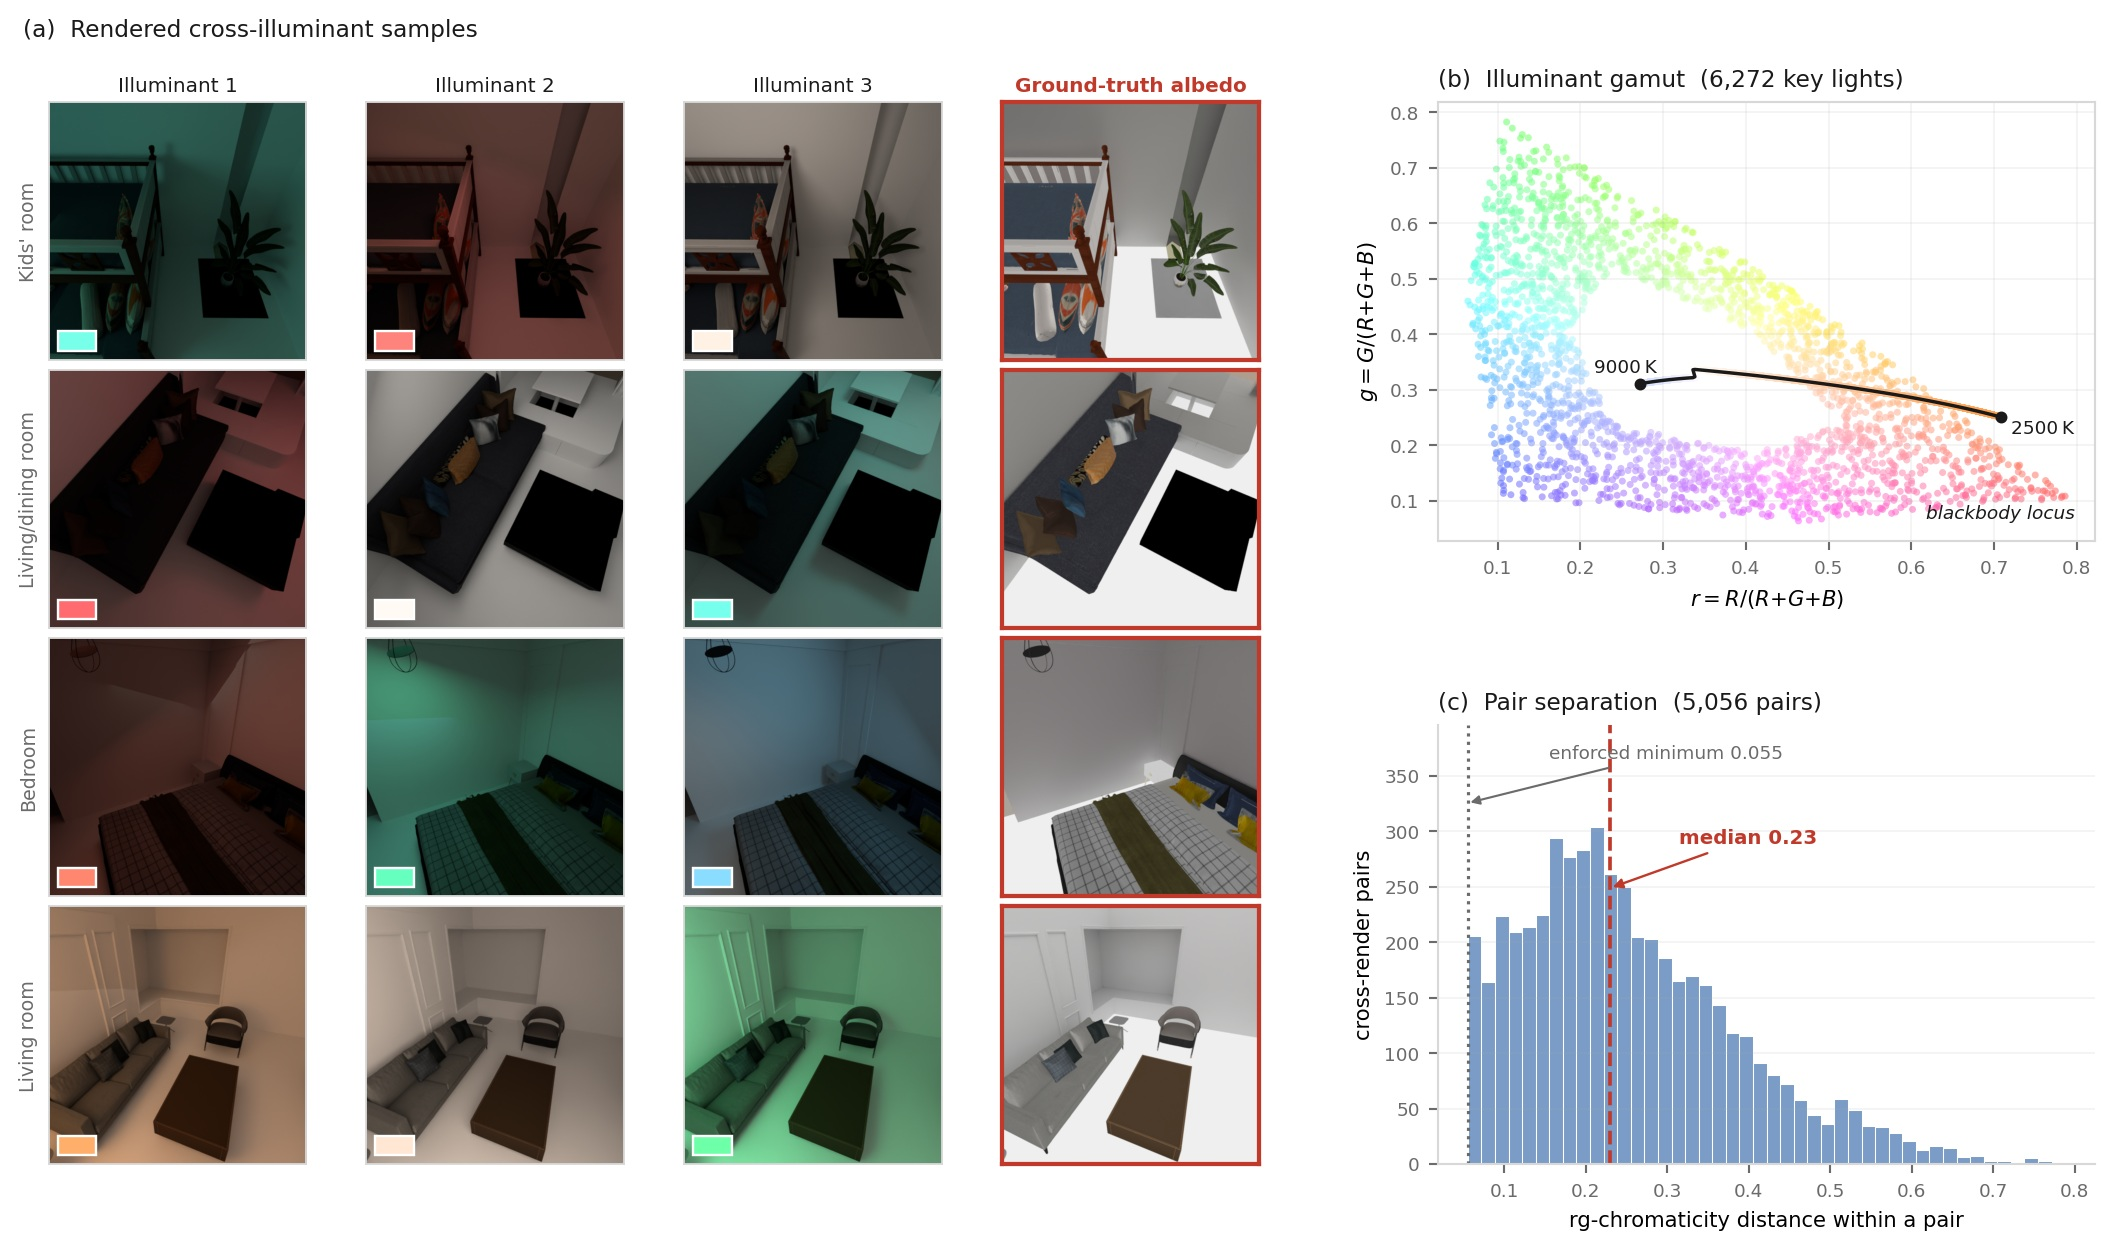
\includegraphics[width=\textwidth]{images/front3d/front3d_dataset.jpg}
  \caption[3D-Front-IID corpus and illuminant distribution.]{%
    3D-Front-IID, the cross-illuminant corpus rendered for this thesis.
    (a) Four rooms, each rendered from a fixed camera under the view's lighting
    variants (the swatch in each panel is that variant's key-light colour), shown
    beside the exact ground-truth albedo obtained from the emission pass. Each
    albedo is pixel-aligned with every lit variant.
    (b) The rg-chromaticity of all 6{,}272 key lights in the corpus, each drawn
    in its own colour, with the blackbody locus overlaid: sampling is deliberately
    not confined to the locus, so the illuminant gamut covers saturated colours
    that natural white-balanced capture never contains.
    (c) The chromaticity distance between the two illuminants of each of the
    5{,}056 cross-render pairs. The renderer enforces a minimum separation, so
    every pair CARI can draw carries a real illuminant-colour change; the median
    separation is $0.23$.
  }
  \label{fig:front3d}
\end{figure}

\section{Optimisation Schedule}
\label{sec:schedule}

Training proceeds in two stages, as illustrated in \figref{fig:curriculum}.

\begin{figure}[t!]
  \centering
  \resizebox{0.95\textwidth}{!}{%
  \begin{tikzpicture}[font=\small, lbl/.style={font=\scriptsize\itshape, align=center}]
    % ── mix bands: x in [0, 12]; Stage A = [0, 5], Stage B = [5, 12] ──
    % Stage A part 1 [0, 3]: Hypersim 1.0
    \fill[gray!30]        (0, 0)   rectangle (3, 1.5);
    % Stage A part 2 [3, 5]: Hypersim 0.6 / InteriorVerse 0.4
    \fill[gray!30]        (3, 0.6) rectangle (5, 1.5);
    \fill[gray!55]        (3, 0)   rectangle (5, 0.6);
    % Stage B [5, 12]: Hypersim 0.4 / MID 0.3 / InteriorVerse 0.3
    \fill[gray!30]        (5, 0.9) rectangle (12, 1.5);
    \fill[myprimary!45]   (5, 0.45) rectangle (12, 0.9);
    \fill[gray!55]        (5, 0)   rectangle (12, 0.45);
    \draw (0, 0) rectangle (12, 1.5);
    \draw (3, 0) -- (3, 1.5);
    \draw[thick] (5, -0.15) -- (5, 1.65);

    % band labels
    \node[lbl] at (1.5, 0.75)  {Hypersim};
    \node[lbl] at (4, 1.05)    {Hypersim};
    \node[lbl] at (4, 0.3)     {IV};
    \node[lbl] at (8.5, 1.2)   {Hypersim};
    \node[lbl] at (8.5, 0.675) {MID raw pairs};
    \node[lbl] at (8.5, 0.225) {InteriorVerse};

    % stage brackets
    \node[align=center] at (2.5, 2.1) {\textbf{Stage A}: synthetic warm-up};
    \node[align=center] at (8.5, 2.1) {\textbf{Stage B}: CARI};

    % timeline axis
    \draw[-latex] (0, -0.5) -- (12.4, -0.5) node[right, font=\scriptsize] {iteration};
    \foreach \x/\t in {0/$t_0$, 3/$t_1$, 5/$t_2$, 12/$T$}
      \draw (\x, -0.42) -- (\x, -0.58) node[below, font=\scriptsize] {\t};

    % checkpoint markers
    \draw[-latex, thick] (5, -1.7) -- (5, -1.0);
    \node[lbl, anchor=north] at (5, -1.7) {baseline checkpoint\\(no CARI, banked)};
    \draw[-latex, thick] (12, -1.7) -- (12, -1.0);
    \node[lbl, anchor=north] at (12, -1.7) {final model};

    % loss activation spans
    \draw[|-|, thick] (0, 3.2) -- (12, 3.2)
      node[midway, above, font=\scriptsize] {supervised + physics + regularisation losses};
    \draw[|-|, thick, red!70!black] (5, 2.55) -- (12, 2.55)
      node[midway, above, font=\scriptsize] {CARI losses ($\mathcal{L}_{\text{inv}}$, $\mathcal{L}_{\text{expl}}$)};
  \end{tikzpicture}}
  \caption[Two-stage training schedule.]{%
    Two-stage training schedule.
    Stage A establishes the supervised baseline on synthetic data (Hypersim,
    later joined by InteriorVerse).
    Stage B resumes from the Stage-A checkpoint and adds MID raw pairs with the
    CARI losses, keeping the synthetic majority as the absolute-colour anchor.
    The Stage-A checkpoint doubles as the no-CARI baseline in the ablation
    study (\secref{sec:ablation}).
  }
  \label{fig:curriculum}
\end{figure}

\paragraph{Stage A: synthetic warm-up}
The model first trains on Hypersim alone, after which InteriorVerse joins the
mix.
Only the supervised, physics, and regularisation losses are active.
This stage gives the model absolute albedo colour and scale \emph{before} any
invariance constraint is applied. This ordering matters because, when applied to an
unanchored model, an invariance loss can be satisfied by collapsing towards
grey, whereas applied to a colour-anchored model it can only be satisfied by
moving the illuminant colour into the shading.
The Stage-A checkpoint is banked as the no-CARI baseline used throughout
\chapref{ch:experiments}.

\paragraph{Stage B: CARI}
Training resumes from the Stage-A checkpoint with the CARI configuration: the
data mix becomes Hypersim / MID / InteriorVerse (with MID and InteriorVerse
each roughly matching Hypersim's share), the raw cross-render pairs enter
through MID, and $\mathcal{L}_{\text{inv}}$/$\mathcal{L}_{\text{expl}}$
activate.
The synthetic majority keeps re-anchoring absolute colour throughout,
preventing drift while the invariance constraint reshapes the colour split.
The end-of-schedule checkpoint is the final model reported in
\chapref{ch:experiments}.
We describe the schedule here by stage rather than by a specific iteration
count, so that every configuration compared in \chapref{ch:experiments} is
held to the same curriculum and the same total training budget.

\paragraph{Optimisation parameters}
We use Adam with a base learning rate of $2 \times 10^{-4}$ and cosine annealing
to $10^{-7}$ over the training horizon; the frozen DINOv2 encoder is excluded
from the optimiser entirely.
Batches of 4 crops at $512 \times 512$ are accumulated over 8 steps (effective
batch size 32), with gradient-norm clipping at 1.0.
All training runs on a single 24\,GB NVIDIA Quadro RTX 6000.

\paragraph{The full-CARI configuration}
The model reported as ``full CARI'' is this architecture trained under the
two-stage schedule above to 50k iterations: Stage~A establishes absolute albedo
colour and shading structure from Hypersim and InteriorVerse, and Stage~B adds
the real MID raw cross-render pairs and activates the cross-render losses
$\mathcal{L}_{\text{inv}}$ and $\mathcal{L}_{\text{expl}}$ together with the wide
colour skip.
Because the cross-render terms require a \emph{second} forward pass on the paired
frame, the CARI stage holds two graphs in memory; on the 24\,GB card this caps
the per-step crop count, which the gradient accumulation above compensates for.
The frozen DINOv2-Large encoder (304\,M parameters) is kept in evaluation mode
throughout, so only the $\sim$18.5\,M decoder-and-head parameters receive
gradients, which is the main reason the whole pipeline fits on a single commodity GPU.
